\subsection{UC24 - Ricerca ristorante}\label{usecase:24}

\begin{figure}[H]
    \centering
    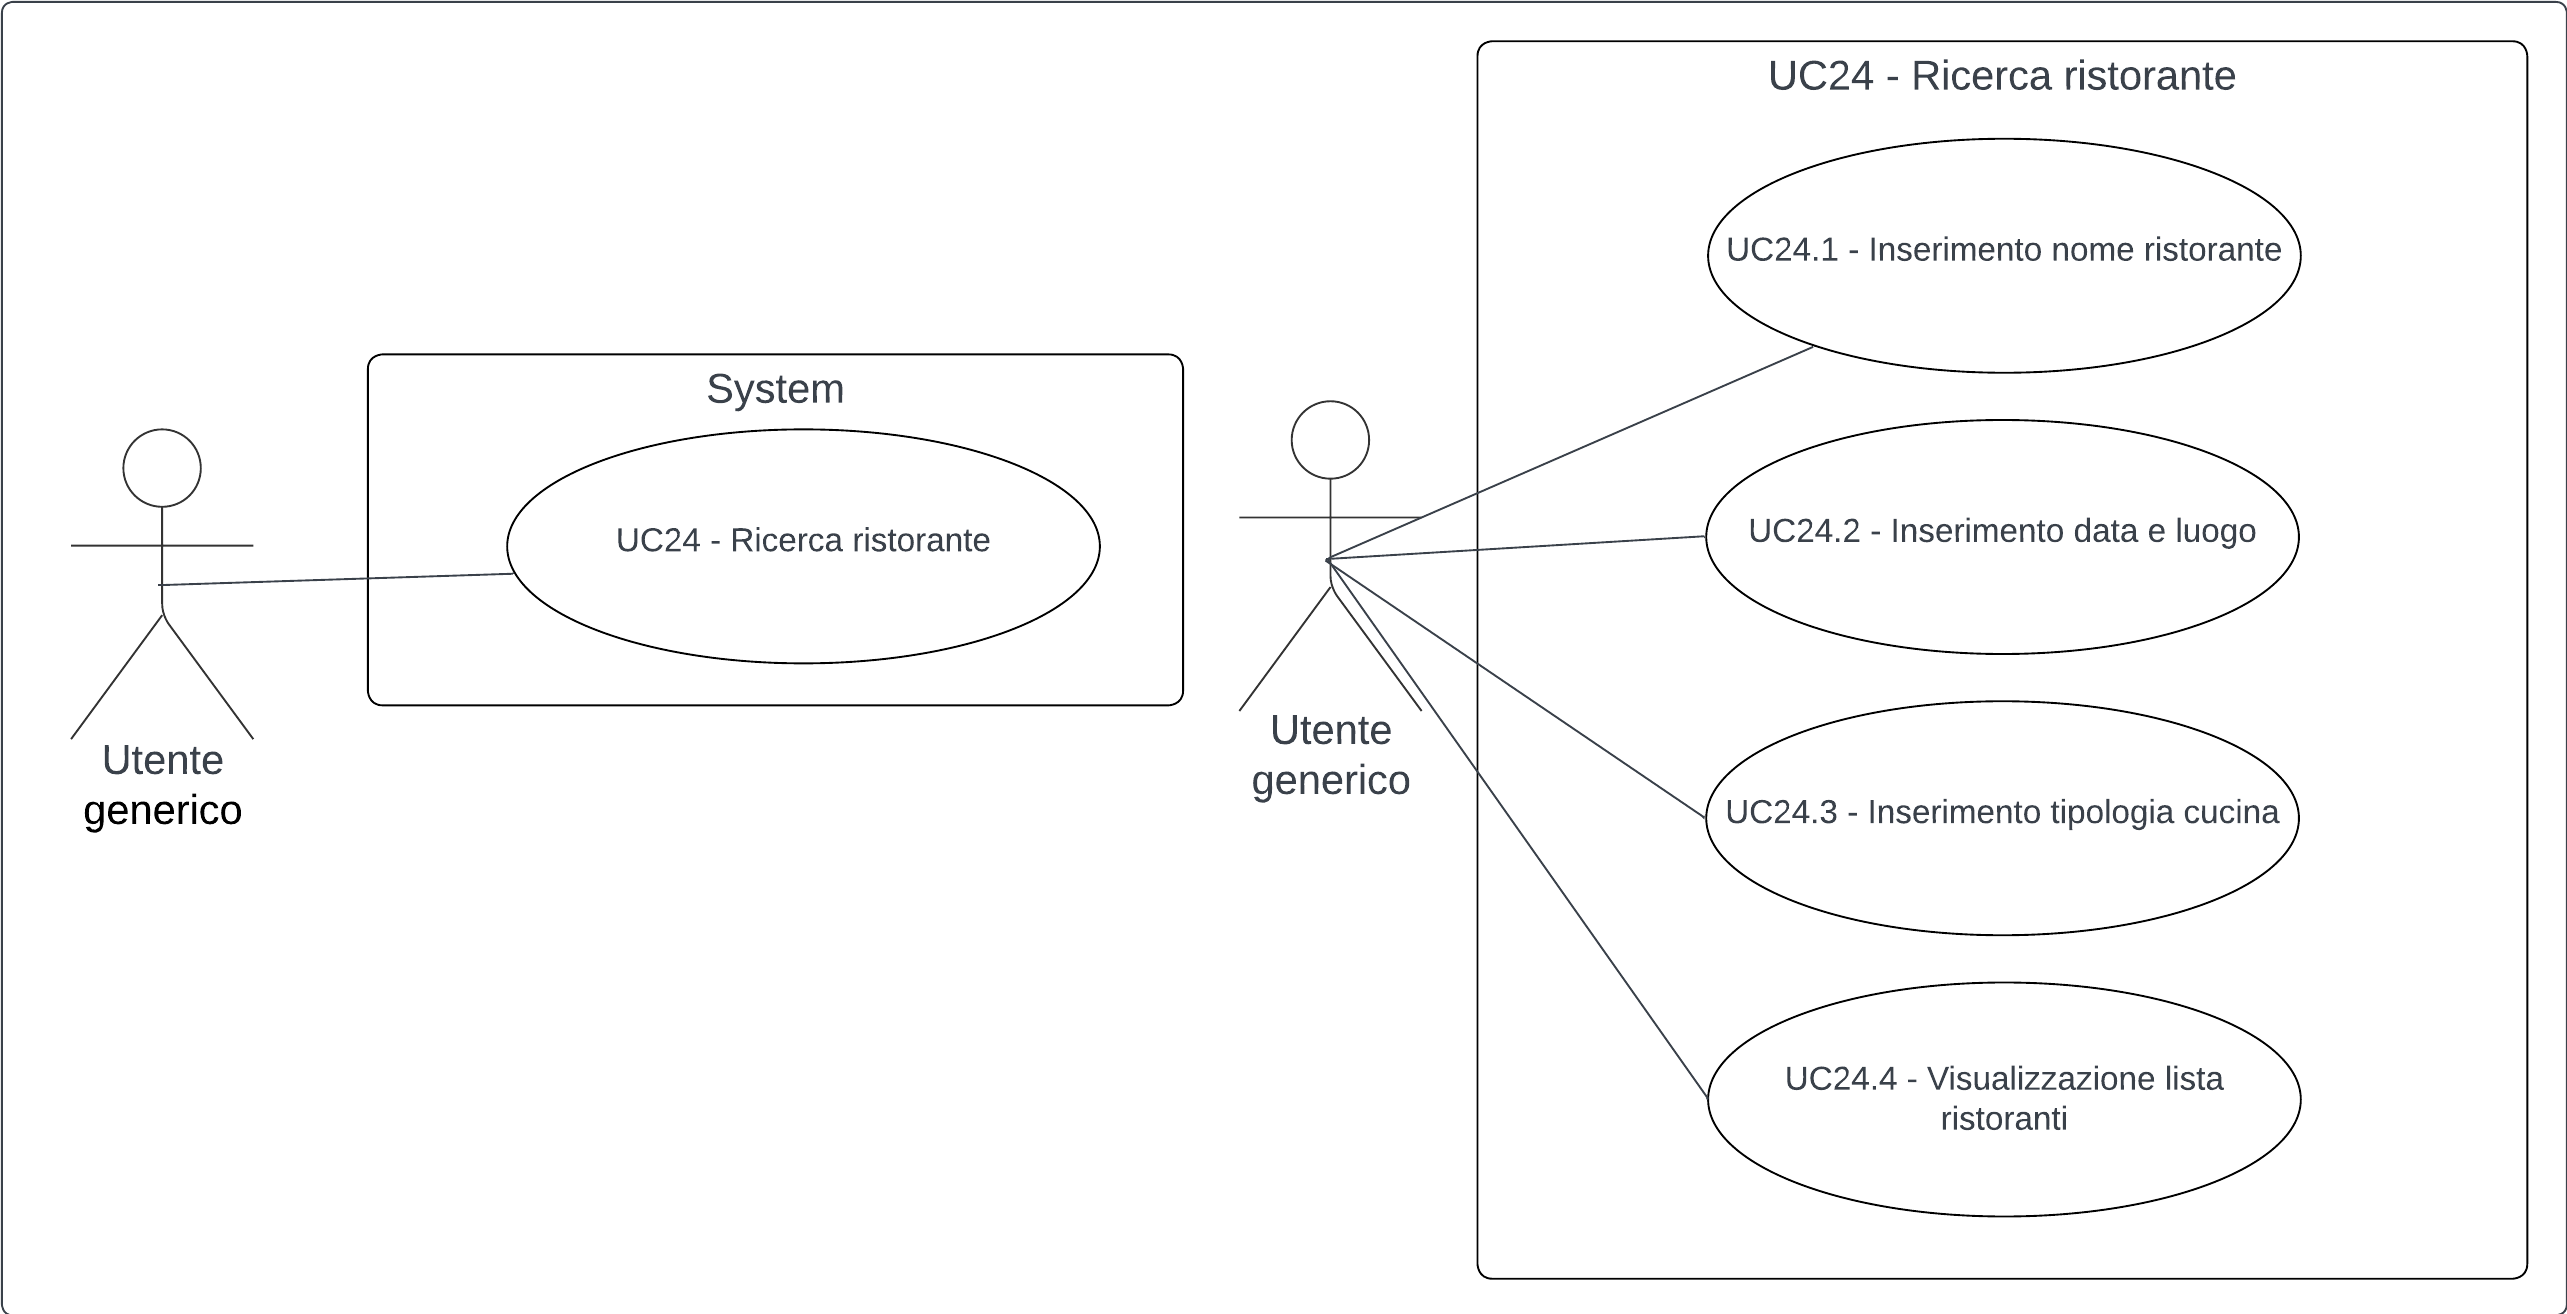
\includegraphics[width=0.9\linewidth]{ucd/UCD24.png}
\end{figure}

\textbf{Attori}:
\begin{itemize}
    \item Utente base autenticato
\end{itemize}
\textbf{Precondizioni}:
\begin{itemize}
    \item L'utente è autenticato come utente base
\end{itemize}
\textbf{Postcondizioni}:
\begin{itemize}
    \item L'utente visualizza una lista di ristoranti che corrispondono ai criteri di ricerca
\end{itemize}
\textbf{Trigger:}
\begin{itemize}
    \item L'utente vuole ricercare un ristorante
\end{itemize}
\textbf{Scenario principale}:
\begin{enumerate}
    \item L'utente può inserire il nome del ristorante.
    \item L'utente inserisce la data per escludere ristoranti chiusi.
    \item L'utente può inserire il luogo.
    \item L'utente può specificare il tipo di cucina.
    \item L'utente conferma.
    \item L'utente visualizza la lista dei ristoranti che rispettano tali criteri.
\end{enumerate}

\subsubsection{UC24.1 - Inserimento nome ristorante
}\label{usecase:24_1}
\textbf{Attori}:
\begin{itemize}
    \item Utente base autenticato
\end{itemize}
\textbf{Precondizioni}:
\begin{itemize}
    \item L'utente è autenticato come utente base.
\end{itemize}
\textbf{Postcondizioni}:
\begin{itemize}
    \item L'utente ha inserito correttamente il nome del ristorante per la ricerca.
\end{itemize}
\textbf{Scenario principale}:
\begin{enumerate}
    \item L'utente inserisce il nome del ristorante che desidera cercare.
\end{enumerate}

\subsubsection{UC24.2 - Inserimento data e luogo
}\label{usecase:24_2}
\textbf{Attori}:
\begin{itemize}
    \item Utente base autenticato
\end{itemize}
\textbf{Precondizioni}:
\begin{itemize}
    \item L'utente è autenticato come utente base.
\end{itemize}
\textbf{Postcondizioni}:
\begin{itemize}
    \item L'utente ha inserito correttamente la data e/o il luogo per la ricerca dei ristoranti.
\end{itemize}
\textbf{Scenario principale}:
\begin{enumerate}
    \item L'utente inserisce la data per escludere i ristoranti chiusi.
    \item L'utente inserisce il luogo desiderato per la ricerca dei ristoranti.
\end{enumerate}


\subsubsection{UC24.3 - Inserimento tipologia cucina
}\label{usecase:24_3}
\textbf{Attori}:
\begin{itemize}
    \item Utente base autenticato
\end{itemize}
\textbf{Precondizioni}:
\begin{itemize}
    \item L'utente è autenticato come utente base.
\end{itemize}
\textbf{Postcondizioni}:
\begin{itemize}
    \item L'utente ha inserito correttamente la tipologia di cucina desiderata per la ricerca dei ristoranti.
\end{itemize}
\textbf{Scenario principale}:
\begin{enumerate}
    \item L'utente specifica il tipo di cucina che desidera cercare nei ristoranti.
\end{enumerate}


\subsubsection{UC24.4 - Visualizzazione lista ristoranti
}\label{usecase:24_4}
\textbf{Attori}:
\begin{itemize}
    \item Utente base autenticato
\end{itemize}
\textbf{Precondizioni}:
\begin{itemize}
    \item L'utente è autenticato come utente base.
    \item L'utente ha inserito correttamente tutti i criteri di ricerca per i ristoranti.
\end{itemize}
\textbf{Postcondizioni}:
\begin{itemize}
    \item L'utente visualizza una lista di ristoranti che corrispondono ai criteri di ricerca.
\end{itemize}
\textbf{Scenario principale}:
\begin{enumerate}
    \item Dopo aver confermato i criteri di ricerca, l'utente visualizza la lista dei ristoranti che rispettano tali criteri.
\end{enumerate}



\newpage